\section{Performance-Messungen der parallelen Implementation}

\subsection{Evaluierung der Optimierungen}

\begin{frame}[allowframebreaks]{Parallele Verarbeitung einzelner Bildpaare}
	\begin{figure}[h]
		%TODO: größer & besser lesbar
		\begin{subfigure}[b]{0.47\textwidth}
			\centering
			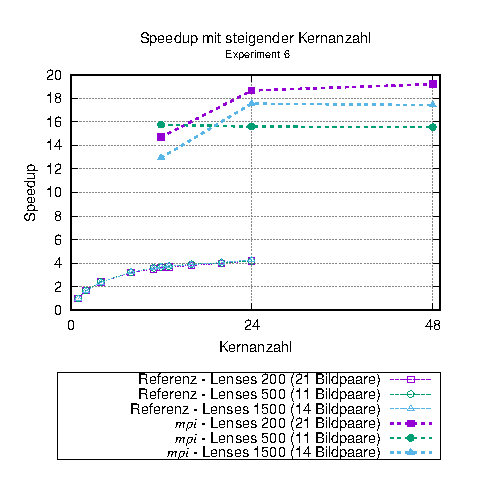
\includegraphics[width=\textwidth]{pdf/mpi_speedup_exp6}
			\caption{Experiment 6}
		\end{subfigure}
		\hfill
		\begin{subfigure}[b]{0.47\textwidth}
			\centering
			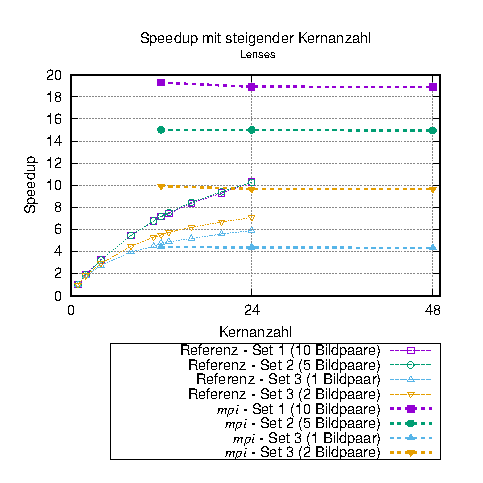
\includegraphics[width=\textwidth]{pdf/mpi_speedup_lenses}
			\caption{Lenses}
		\end{subfigure}
		\caption{Speed-Up \textit{mpi} gegenüber Referenz}
	\end{figure}
	
	\framebreak
	
	\begin{figure}[h]
		\begin{subfigure}[b]{0.47\textwidth}
			\centering
			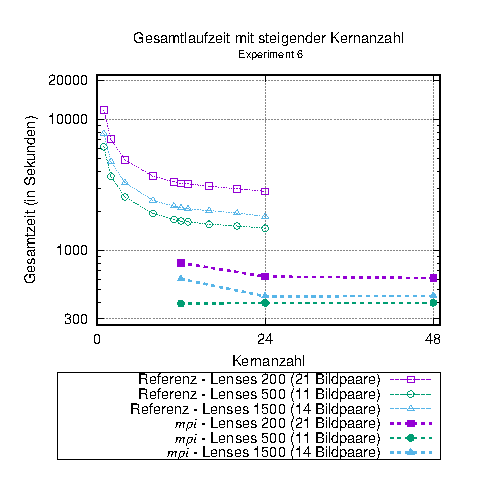
\includegraphics[width=\textwidth]{pdf/mpi_times_exp6}
			\caption{Experiment 6}
		\end{subfigure}
		\hfill
		\begin{subfigure}[b]{0.47\textwidth}
			\centering
			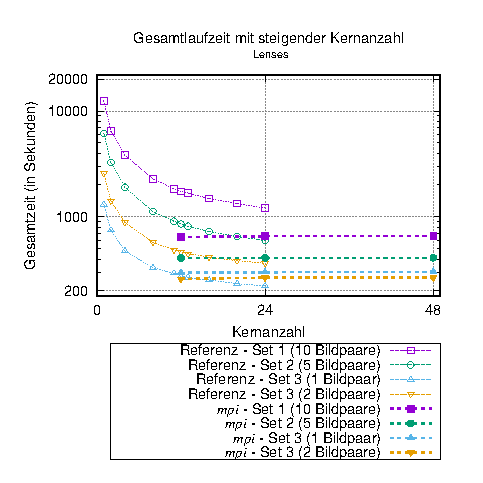
\includegraphics[width=\textwidth]{pdf/mpi_times_lenses}
			\caption{Lenses}
		\end{subfigure}
		\caption{Speed-Up \textit{mpi} gegenüber Referenz}
	\end{figure}
\end{frame}

\begin{frame}[allowframebreaks]{Parallele Verarbeitung innerhalb einzelner Bildpaare}
	%TODO: größer & besser lesbar
	\begin{figure}[h]
		\begin{subfigure}[b]{0.47\textwidth}
			\centering
			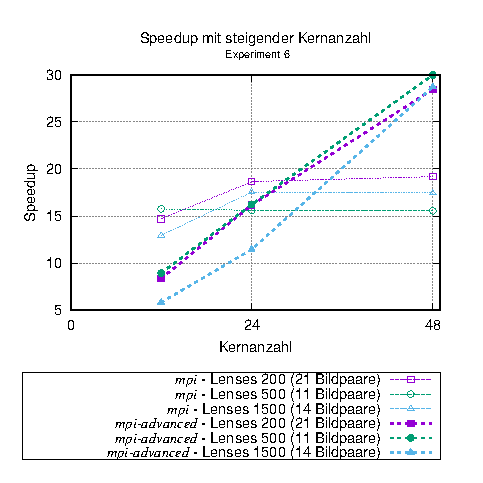
\includegraphics[width=\textwidth]{pdf/mpi_advanced_speedup_exp6}
			\caption{Experiment 6}
		\end{subfigure}
		\hfill
		\begin{subfigure}[b]{0.47\textwidth}
			\centering
			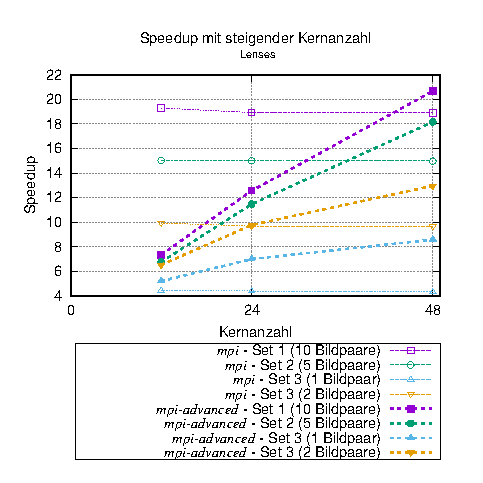
\includegraphics[width=\textwidth]{pdf/mpi_advanced_speedup_lenses}
			\caption{Lenses}
		\end{subfigure}
		\caption{Speed-Up \textit{mpi-advanced} gegenüber \textit{mpi}}
	\end{figure}
	
	\framebreak
	
	\begin{figure}[h]
		\begin{subfigure}[b]{0.47\textwidth}
			\centering
			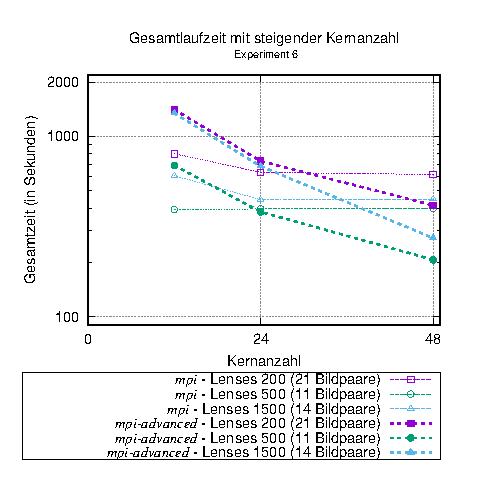
\includegraphics[width=\textwidth]{pdf/mpi_advanced_times_exp6}
			\caption{Experiment 6}
		\end{subfigure}
		\hfill
		\begin{subfigure}[b]{0.47\textwidth}
			\centering
			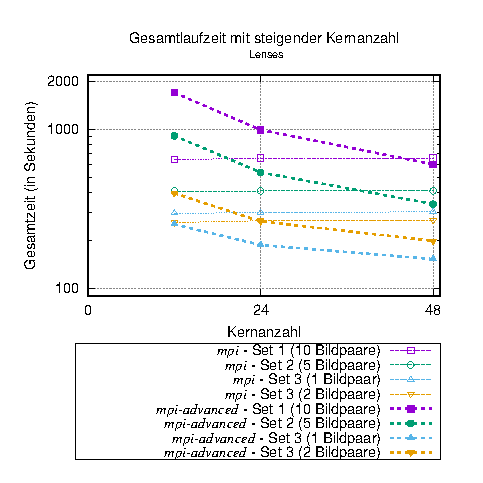
\includegraphics[width=\textwidth]{pdf/mpi_advanced_times_lenses}
			\caption{Lenses}
		\end{subfigure}
		\caption{Speed-Up \textit{mpi-advanced} gegenüber \textit{mpi}}
	\end{figure}
\end{frame}

\begin{frame}{Nutzen optimierter Bibliotheken}
	%TODO: dickerer roter Strich
	\begin{figure}[h]
		\begin{subfigure}[b]{0.47\textwidth}
			\centering
			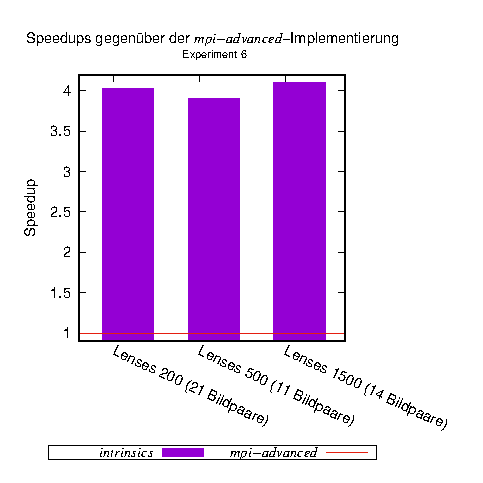
\includegraphics[width=\textwidth]{pdf/speedups_intrinsics_exp6}
			\caption{Experiment 6}
		\end{subfigure}
		\hfill
		\begin{subfigure}[b]{0.47\textwidth}
			\centering
			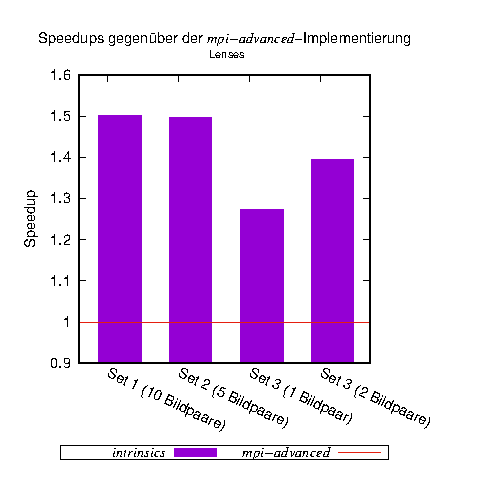
\includegraphics[width=\textwidth]{pdf/speedups_intrinsics_lenses}
			\caption{Lenses}
		\end{subfigure}
		\caption{Speed-Up \textit{intrinsics} gegenüber \textit{mpi-advanced} (mit zwölf Kernen)}
	\end{figure}
\end{frame}


\begin{frame}{Kompilieren}
	%TODO: dickerer roter Strich
	\begin{figure}[h]
		\begin{subfigure}[b]{0.47\textwidth}
			\centering
			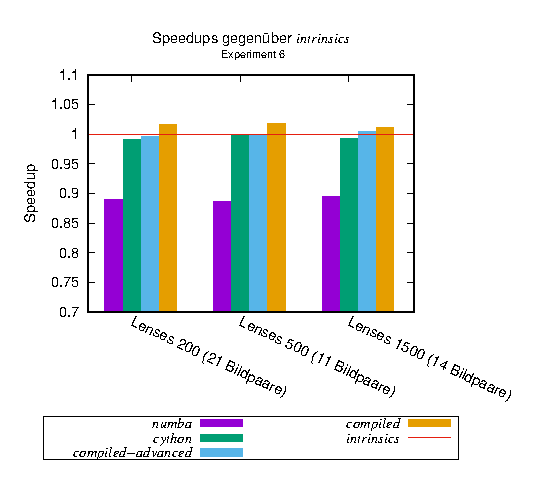
\includegraphics[width=\textwidth]{pdf/speedups_exp6}
			\caption{Experiment 6}
		\end{subfigure}
		\hfill
		\begin{subfigure}[b]{0.47\textwidth}
			\centering
			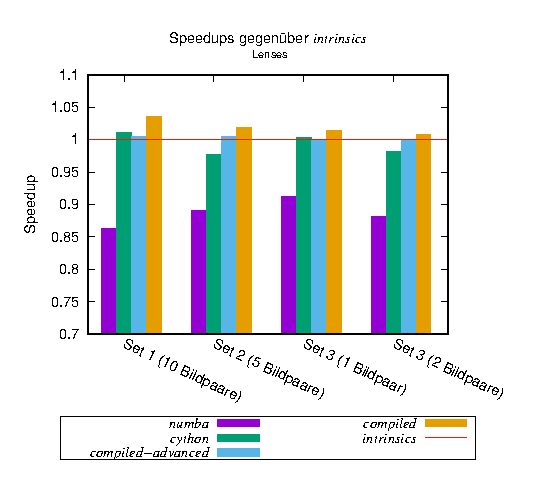
\includegraphics[width=\textwidth]{pdf/speedups_lenses}
			\caption{Lenses}
		\end{subfigure}
		\caption{Speed-Ups gegenüber \textit{intrinsics} (mit zwölf Kernen)}
	\end{figure}
\end{frame}

\subsection{Skalierung}
\begin{frame}{Skalierung}
	%TODO: größer & besser lesbar
	\begin{center}
		\begin{figure}[h]
			\begin{subfigure}[b]{0.45\textwidth}
				\centering
				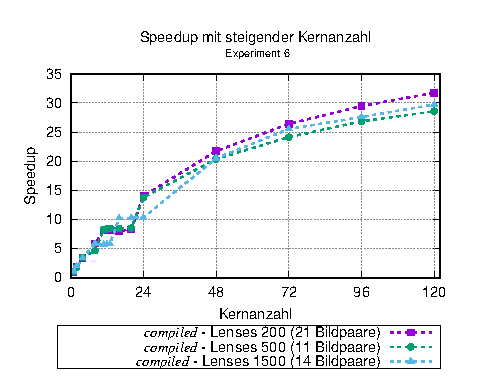
\includegraphics[width=\textwidth]{pdf/best_speedup_exp6_standalone}
				\caption{Experiment 6}
			\end{subfigure}
			\hfill
			\begin{subfigure}[b]{0.45\textwidth}
				\centering
				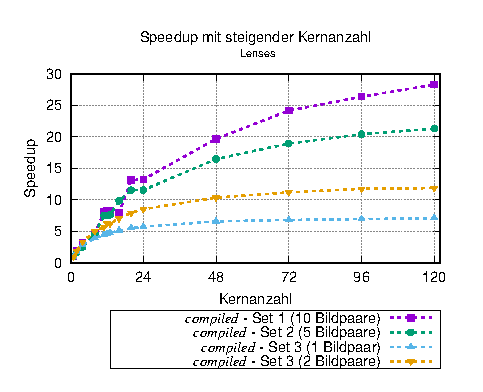
\includegraphics[width=\textwidth]{pdf/best_speedup_lenses_standalone}
				\caption{Lenses}
			\end{subfigure}
			\caption{Speed-Up der \textit{compiled} Implementierung}
		\end{figure}
	\end{center}
\end{frame}
